\documentclass{report}
\usepackage[T1]{fontenc}
\usepackage{graphicx}
\usepackage[top=1in, bottom=1in, right=1in, left=1in]{geometry}
\usepackage{parskip}
\usepackage{pdfpages}

\usepackage{ragged2e}
\usepackage{mwe}

\setlength{\RaggedRightParfillskip}{.25\textwidth plus 1fil}
\setlength{\RaggedRightRightskip}{0pt plus .1\textwidth}
\setlength{\RaggedRightParindent}{4em}

\begin{document}
	\fontfamily{lmtt}\selectfont
    \RaggedRight
    \section*{Introduction}
    \vspace{-0.1cm}\hrule\vspace{0.2cm}
    \par{\indent Flowcell sensors have many applications; disease detection, refractive index measuring, and reactivity measuring to name a few. These sensors have been operating on the basis of electromagnetic surface phenomena for decades. Most flowcells on the market work by exploiting surface plasma oscillations (SPOs). These oscillations are highly sensitive to changes in the optical properties of the adjacent medium and follow from Maxwell's equations when the dielectric functions of each medium satisfies
    \[
        \frac{\epsilon_{spo}}{\epsilon_{adjacent}} < -1
    \]
		Metals like aluminum, copper, gold, and silver have negative dielectric functions at wavelengths in the red/infrared, so films of these metals are used as to generate SPOs in most flowcell sensors via a process known as Surface Plasmon Resonance (SPR). There are quite a few drawbacks for using metal films, however. Metals are highly reactive so they require regular maintenance. These films also require particular wavelengths of incident light to excite the oscillations. Rather than using metal films, one-dimensional photonic crystals, or multilayers, can be designed to exhibit the phenomenon of surface electromagnetic waves (SEWs) or Bloch surface waves (BSWs), named after the physicist Felix Bloch who was famous for working with periodic systems. These surface waves have the same practical application as SPOs. Multilayers overcome both of the shortcomings of metal films listed here. They can be designed to work for any wavelength and are typically made of nonreactive glass. In addition to these benefits, we expect that our 3-D printed and multilayer-based flowcell sensor will be more sensitive and precise with its measurements and be far cheaper to both build and maintain compared to traditional SPR sensors.}


			\par{To take measurements with our sensor we look at the reflected image of incident laser light. Our multilayer is designed to trap incident light in the last layer at a critical angle; this results in a dark band in our reflected image. A diagram of the process is shown below.}
\newline	
	\begin{figure}[h!]
		\raisebox{-0.5\height}{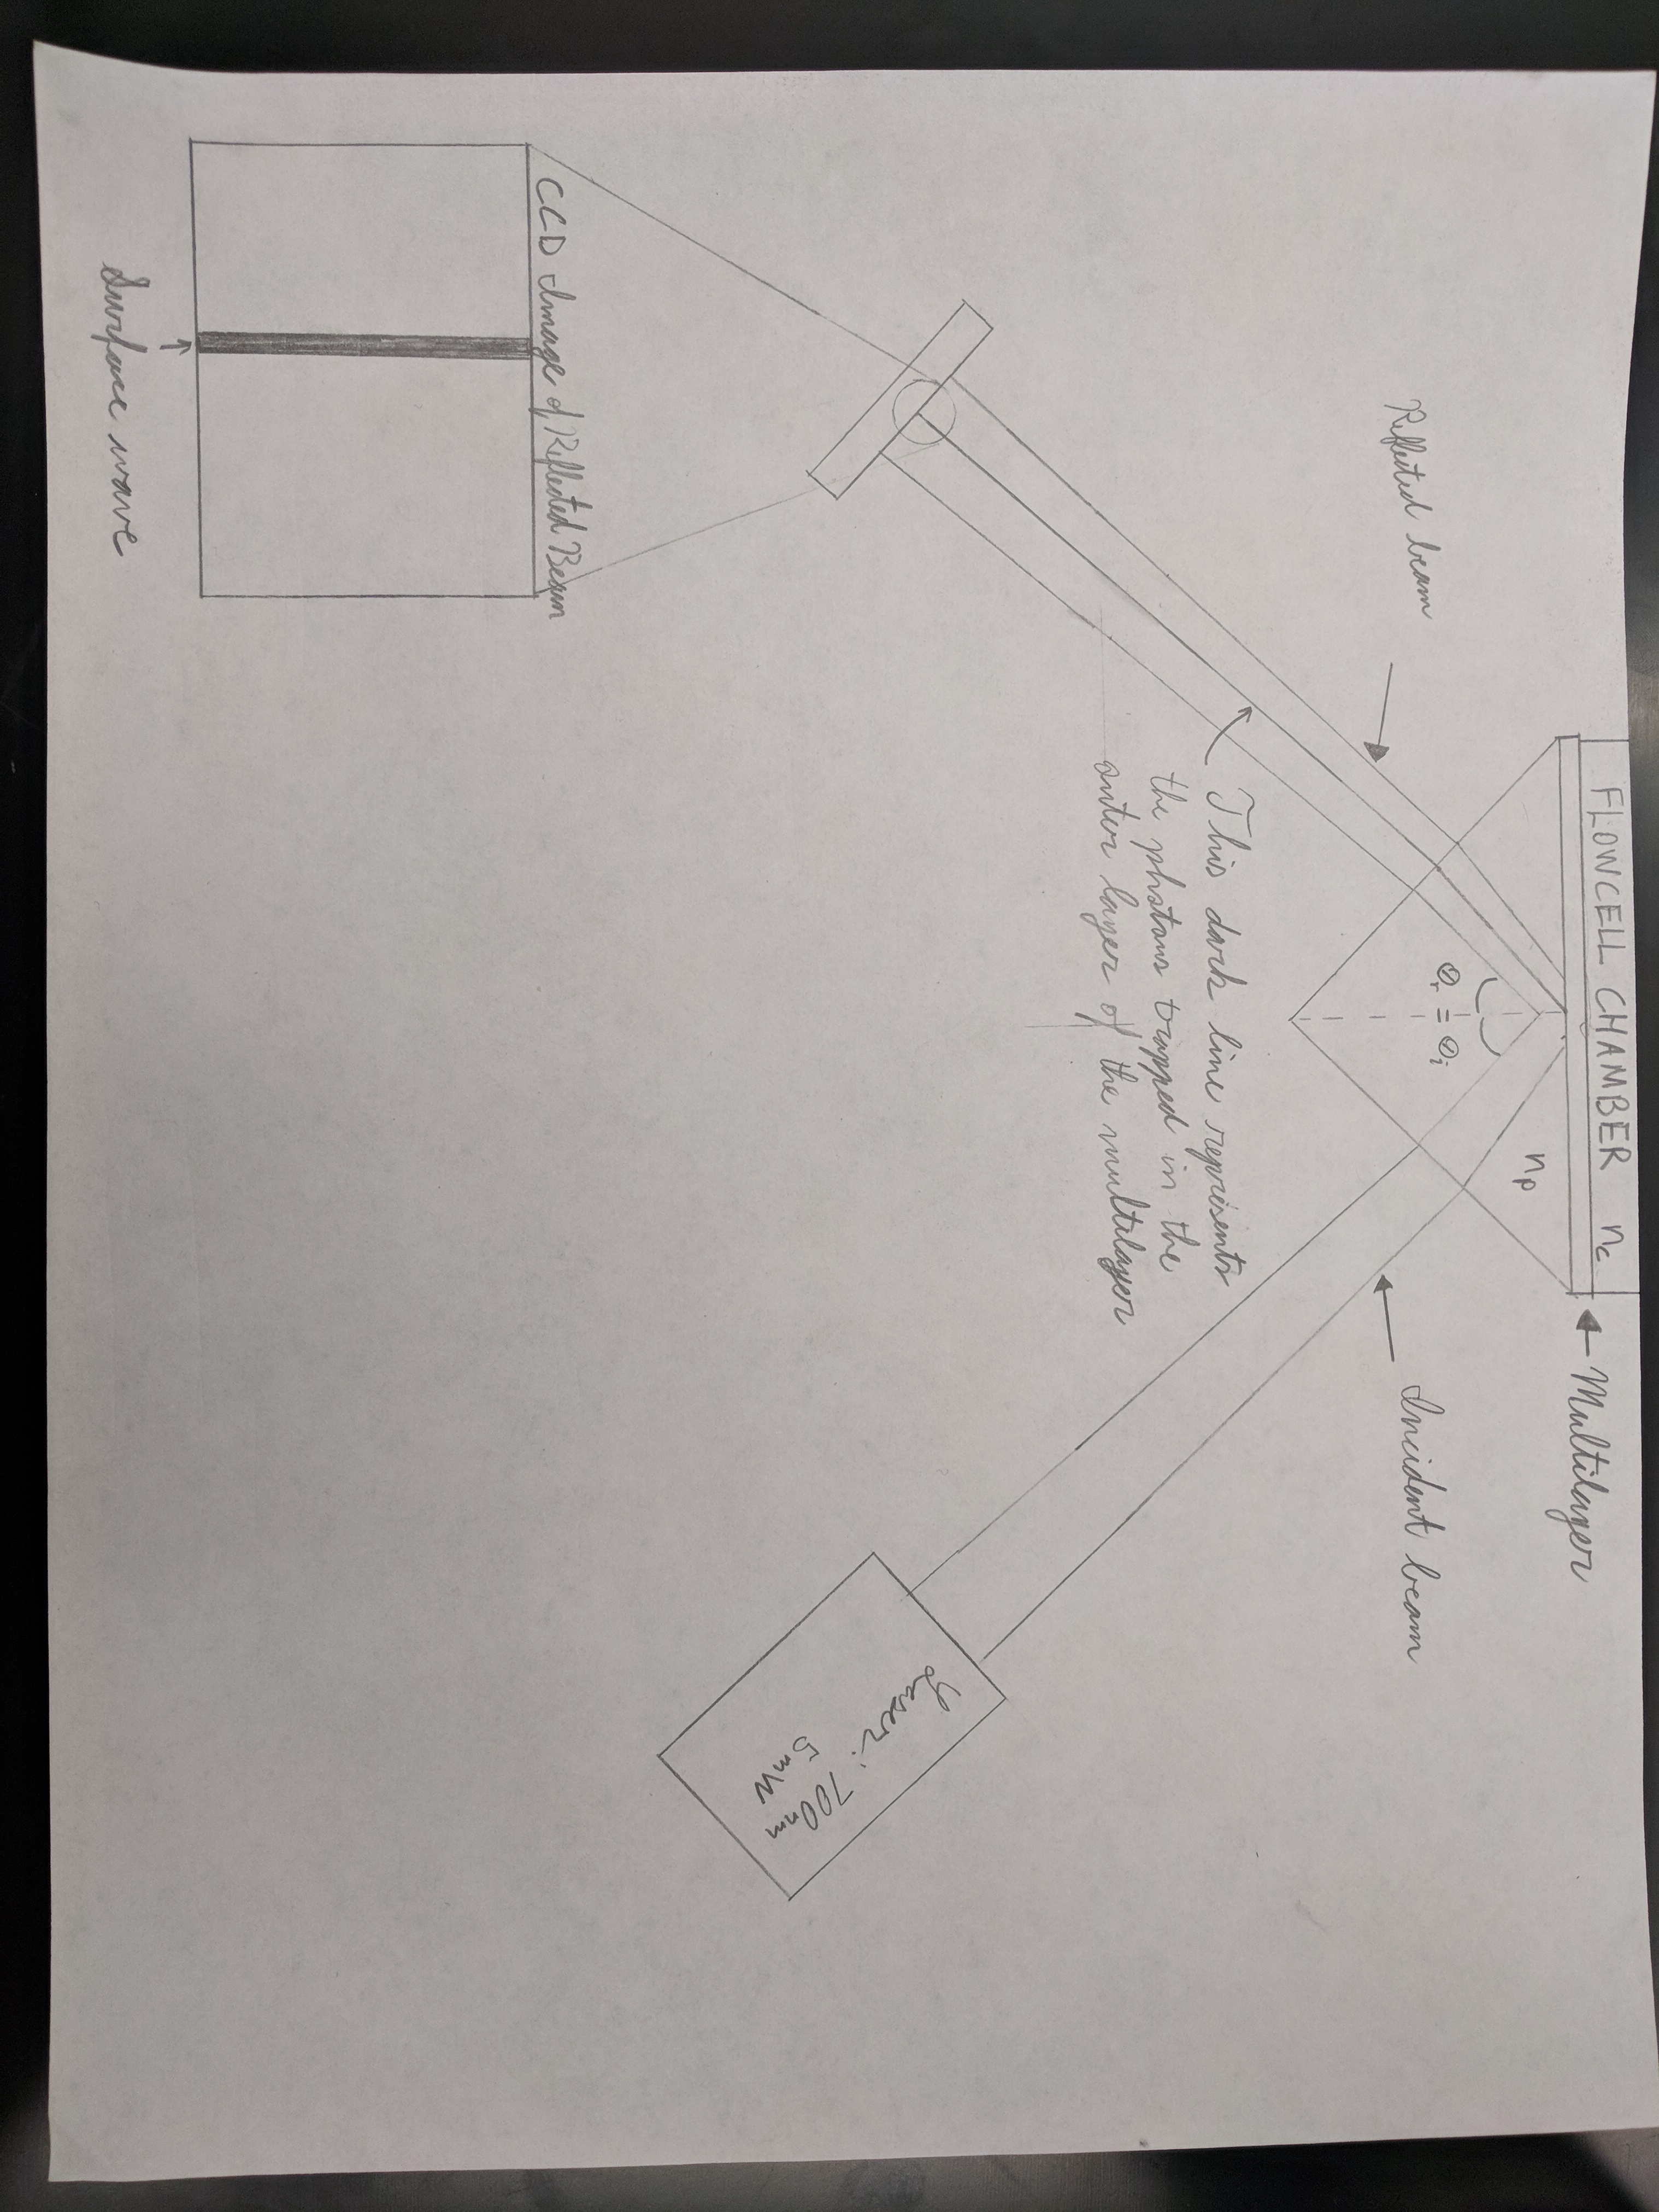
\includegraphics[height=\linewidth, angle=90, origin=c]{media/setup_diagram.jpg}}
	\end{figure}

	\par{As fluids or gases are put into the flowcell chamber the index of refraction, $n_c$, changes. The condition for total internal reflection, found from Snell's law, for the interface between a glass prism and some transmitting medium whose index of refraction varies with time is given by:}
	\[
			\sin{\theta_c} = \frac{n_t(t)}{n_g}
	\]

	\par{We obtain an expression for the angle of reflection as a function of time by the Law of Reflection:}
	\[
			\theta_r(t) = \arcsin{\frac{n_t(t)}{n_g}}
	\]


	\par{\indent Note that this expression is for a single interface and hence does not accurately reflect our setup as we have a glass prism and a multilayer. With that said, this expression for $\theta_r$ does capture the essence of our setup; the reflected angle is a function of the index of refraction of the transmission. Using this fact we can associate variations in the flowcell chamber's index of refraction with differences in the angle of reflectance. These angular differences can be calculated by tracking the variation in the position of the dark band in the reflected image.}
	\newline
	\begin{figure}[h!]
		\raisebox{-0.5\height}{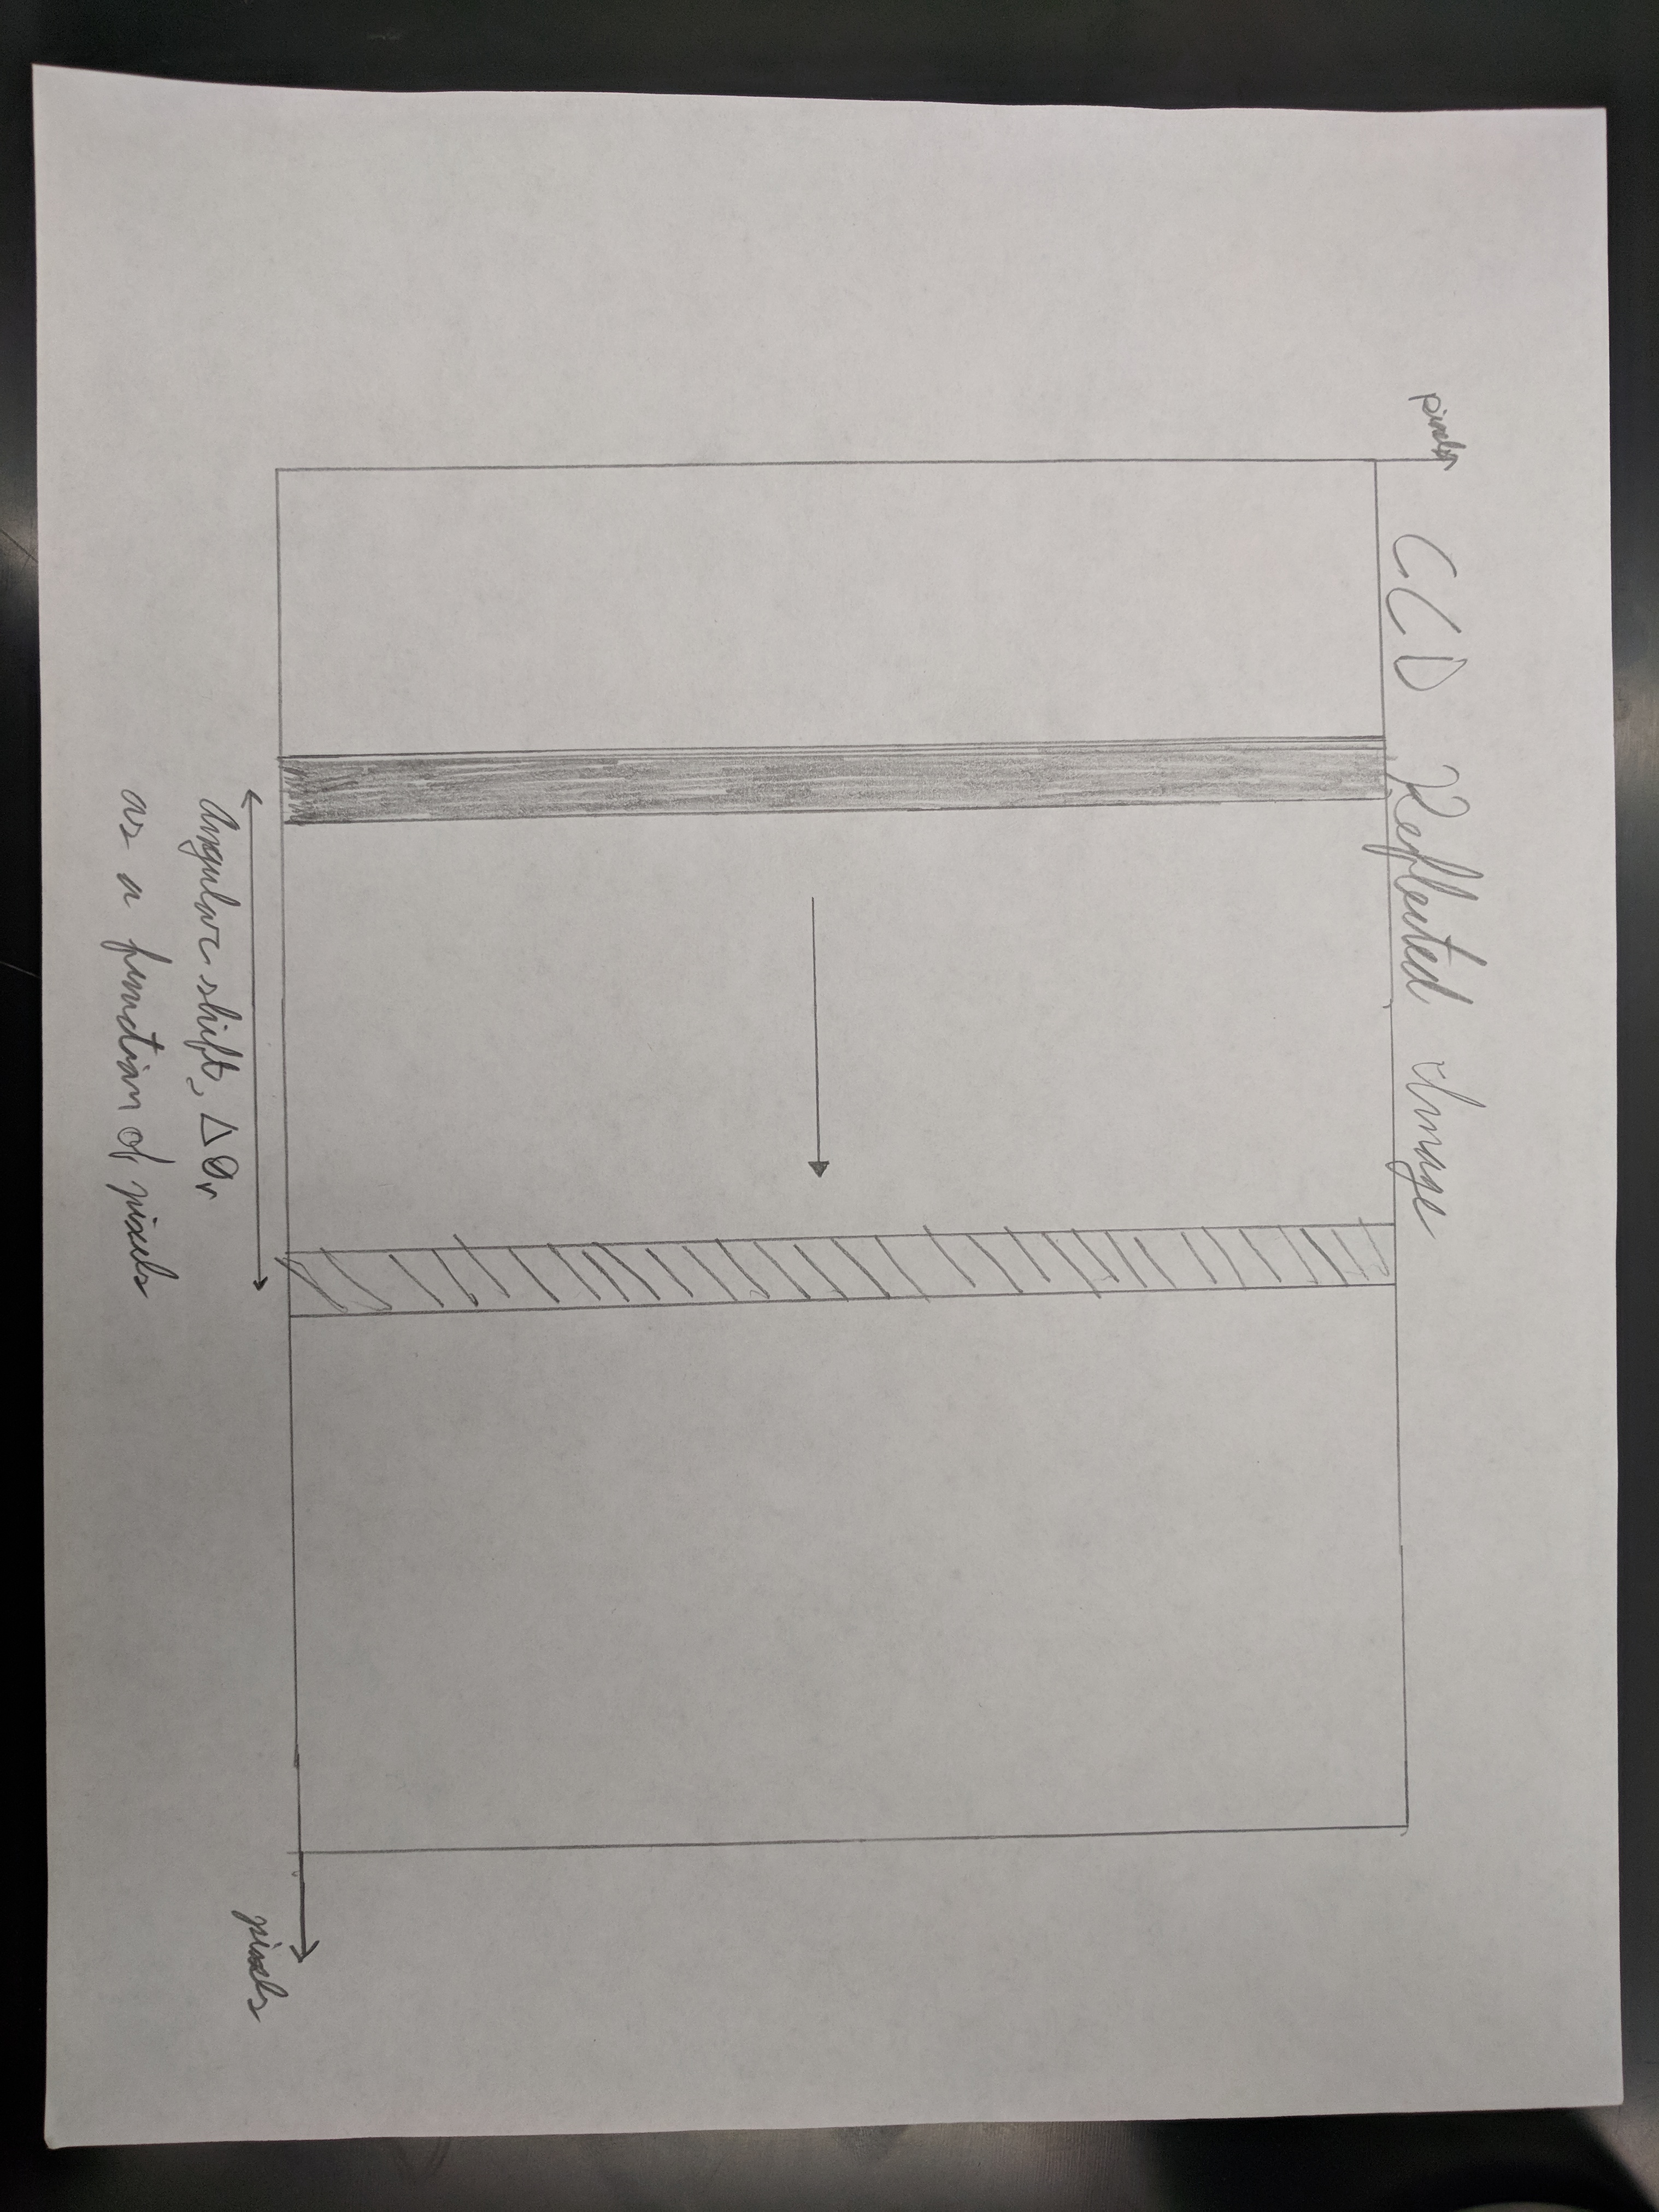
\includegraphics[height=\linewidth, angle=90, origin=c]{media/angular_sep.jpg}}
	\end{figure}
	\vspace{-3cm}
	\pagebreak
	\par{\indent Now with an an expression for the rate of change of reflected angle we can measure the index of refraction inside the flowcell chamber over time. From this data we can interpolate the mutual reactivity between molecules in a reaction, or maybe the rate of mixing of sugar water at a given temperature.

\end{document}
